\begin{frame}
  \frametitle{Dataset overview}
  
  \begin{figure}[tbph]
    \centering
    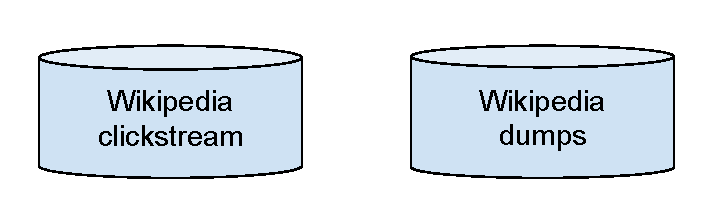
\includegraphics[width=0.7\linewidth]{images/datasets}
  \end{figure}
  
\end{frame}

\begin{frame}
  \frametitle{Clickstream}
  \begin{figure}[tbph]
    \centering
    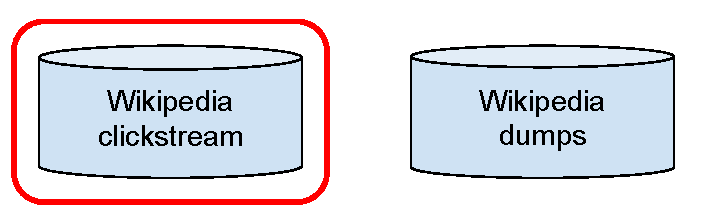
\includegraphics[width=0.7\linewidth]{images/datasets_wc}
  \end{figure}
  
  \begin{itemize}
    \item \textit{(referer, resource)}-pairs of articles -- and more!
    \item Counts user navigation between pairs
    \item Noisy data (crawlers, spoofing, etc.)
    \item Privacy limitation (10-rule)
    \item Monthly dumps (not every month)
    \item March 16': 6.8 billion requests, 25 million pairs
  \end{itemize}
  
\end{frame}

\begin{frame}
  \frametitle{Wikipedia dumps}
  \begin{figure}[tbph]
    \centering
    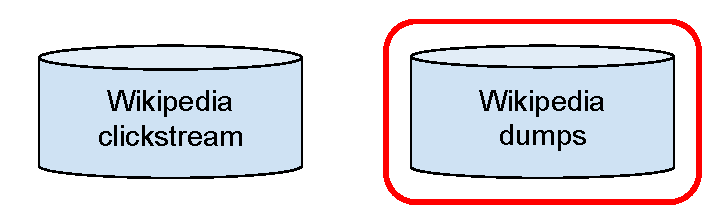
\includegraphics[width=0.7\linewidth]{images/datasets_wd}
  \end{figure}
  
  \begin{itemize}
    \item Dump of articles from English Wikipedia
    \item Contains $>5$ millions articles
    \item Released once a month
    \item XML format
    \item $\approx$ 50GB textual data
  \end{itemize}
  
\end{frame}



% slide 8: overview listing datasets we used
% slide 9: Wiki dumps
% slide 10: wiki clickstream